%%%%%%%%%%%%%%%%%%%%%%%%%%%%%%%%%%%%%%%%%
% Beamer Presentation
% LaTeX Template
% Version 1.0 (10/11/12)
%
% This template has been downloaded from:
% http://www.LaTeXTemplates.com
%
% License:
% CC BY-NC-SA 3.0 (http://creativecommons.org/licenses/by-nc-sa/3.0/)
%
%%%%%%%%%%%%%%%%%%%%%%%%%%%%%%%%%%%%%%%%%

%----------------------------------------------------------------------------------------
%   PACKAGES AND THEMES
%----------------------------------------------------------------------------------------
\documentclass[aspectratio=169]{beamer}
\usepackage{multicol}
\usepackage{tikz, pgfplots}
\usepackage{enumitem}
\pgfplotsset{compat=1.5.1}
\usepgfplotslibrary{fillbetween}
\usepackage{tcolorbox}
\resetcounteronoverlays{saveenumi}
\newcounter{saveenumi}
\newcommand{\seti}{\setcounter{saveenumi}{\value{enumi}}}
\newcommand{\conti}{\setcounter{enumi}{\value{saveenumi}}}

\setbeamercovered{transparent}
%\usepackage{enumitem}
\mode<presentation> {

% The Beamer class comes with a number of default slide themes
% which change the colors and layouts of slides. Below this is a list
% of all the themes, uncomment each in turn to see what they look like.

%\usetheme{default}
%\usetheme{AnnArbor}
%\usetheme{Antibes}
%\usetheme{Bergen}
%\usetheme{Berkeley}
%\usetheme{Berlin}
%\usetheme{Boadilla}
%\usetheme{CambridgeUS}
%\usetheme{Copenhagen}
%\usetheme{Darmstadt}
%\usetheme{Dresden}
%\usetheme{Frankfurt}
%\usetheme{Goettingen}
%\usetheme{Hannover}
\usetheme{Ilmenau}
%\usetheme{JuanLesPins}
%\usetheme{Luebeck}
%\usetheme{Madrid}
%\usetheme{Malmoe}
%\usetheme{Marburg}
%\usetheme{Montpellier}
%\usetheme{PaloAlto}
%\usetheme{Pittsburgh}
%\usetheme{Rochester}
%\usetheme{Singapore}
%\usetheme{Szeged}
%\usetheme{Warsaw}

% As well as themes, the Beamer class has a number of color themes
% for any slide theme. Uncomment each of these in turn to see how it
% changes the colors of your current slide theme.

%\usecolortheme{albatross}
%\usecolortheme{beaver}
%\usecolortheme{beetle}
%\usecolortheme{crane}
%\usecolortheme{dolphin}
%\usecolortheme{dove}
%\usecolortheme{fly}
%\usecolortheme{lily}
%\usecolortheme{orchid}
%\usecolortheme{rose}
%\usecolortheme{seagull}
%\usecolortheme{seahorse}
%\usecolortheme{whale}
%\usecolortheme{wolverine}

%\setbeamertemplate{footline} % To remove the footer line in all slides uncomment this line
%\setbeamertemplate{footline}[page number] % To replace the footer line in all slides with a simple slide count uncomment this line
\usefonttheme[onlymath]{serif}

\setbeamertemplate{navigation symbols}{} % To remove the navigation symbols from the bottom of all slides uncomment this line
}
\definecolor{blizzardblue}{rgb}{0.67, 0.9, 0.93}
\newcommand{\Cross}{$\mathbin{\tikz [x=1.4ex,y=1.4ex,line width=.2ex] \draw (0,0) -- (1,1) (0,1) -- (1,0);}$}%

\usepackage{graphicx} % Allows including images
\usepackage{booktabs} % Allows the use of \toprule, \midrule and \bottomrule in tables
\usepackage{mathtools}
\AtBeginSection[]{
	\begin{frame}
		\vfill
		\centering
		\begin{beamercolorbox}[sep=8pt,center,shadow=true,rounded=true]{title}
			\usebeamerfont{title}\insertsectionhead\par%
		\end{beamercolorbox}
		\vfill
	\end{frame}
}

%\usepackage{enumitem}

%----------------------------------------------------------------------------------------
%   TITLE PAGE
%----------------------------------------------------------------------------------------

\title[Signals and Systems - Tutorial \#2]{The $z$ -Transform} % The short title appears at the bottom of every slide, the full title is only on the title page

\author{Amirhossein Afsharrad} % Your name

\institute[Sharif University of Technology] % Your institution as it will appear on the bottom of every slide, may be shorthand to save space
{
Signals and Systems\\ 
Tutorial Session 2\\ 
\medskip
 % Your email address
}

\date{\today} % Date, can be changed to a custom date

\begin{document}

\begin{frame}
\titlepage % Print the title page as the first slide
\end{frame}

\begin{frame}
\frametitle{Overview} % Table of contents slide, comment this block out to remove it
\tableofcontents % Throughout your presentation, if you choose to use \section{} and \subsection{} commands, these will automatically be printed on this slide as an overview of your presentation
\end{frame}

%----------------------------------------------------------------------------------------
%   PRESENTATION SLIDES
%----------------------------------------------------------------------------------------

%------------------------------------------------
\section{Introduction} 

\begin{frame}
\frametitle{Introduction}
\begin{block}{Definition}
	The $ z $-transform of a discrete-time signal $ x[n] $ is:
		\[X(z) = \sum_{n=-\infty}^{\infty}x[n]z^{-n} \quad  , \quad z\in\mathbb{C}\]
\end{block}
\end{frame}

\begin{frame}
	\frametitle{Example \#1}
		\begin{align*}
		\only<1-> {x_1[n] &= a^nu[n]\\}
		\only<1> {X_1(z) &= \\}
		\only<2-> {X_1(z) &= \sum_{n=-\infty}^{\infty}x[n]z^{-n}\\}
		\only<3-> {&= \sum_{n=-\infty}^{\infty}a^nu[n]z^{-n}\\}
		\only<4-> {&= \sum_{n=0}^{\infty}a^nz^{-n}\\}
		\only<5> {&= \frac{1}{1-az^{-1}}\\}
		\only<6> {&= \frac{1}{1-az^{-1}} \quad , \quad \textcolor{red}{|az^{-1}|<1}\\}
		\only<7> {&= \frac{1}{1-az^{-1}} \quad , \quad \textcolor{red}{|z|>|a|}\\}
		\end{align*}
\end{frame}

\begin{frame}
	\frametitle{Example \#2}
			\begin{align*}
		\only<1-> {x_2[n] &= -a^nu[-n-1]\\}
		\only<1> {X_2(z) &= \\}
		\only<2> {X_2(z) &= \sum_{n=-\infty}^{\infty}x[n]z^{-n}\\}
		\only<3-> {X_2(z) &= \sum_{n=-\infty}^{\infty}x[n]z^{-n}= \sum_{n=-\infty}^{\infty}-a^nu[-n-1]z^{-n}\\}
%		\only<3-5> {&= \sum_{n=-\infty}^{\infty}-a^nu[-n-1]z^{-n}\\}
		\only<4> {&= \sum_{n=-\infty}^{-1}-a^nz^{-n}\\}
		\only<5-> {&= \sum_{n=-\infty}^{-1}-a^nz^{-n}= \sum_{n=1}^{\infty}-a^{-n}z^{n}\\}
%		\only<5> {&= \sum_{n=1}^{\infty}-a^{-n}z^{n}\\}
%		\only<6-> {X(z) &= \sum_{n=-\infty}^{\infty}x[n]z^{-n}= \sum_{n=-\infty}^{\infty}-a^nu[-n-1]z^{-n}= \sum_{n=-\infty}^{-1}-a^nz^{-n}= \sum_{n=1}^{\infty}-a^{-n}z^{n}\\}
		\only<6-> {&= \frac{-a^{-1}z}{1-a^{-1}z}\\}
		\only<7> {&= \frac{1}{1-az^{-1}}\\}
		\only<8> {&= \frac{1}{1-az^{-1}}\quad , \quad \textcolor{red}{|a^{-1}z|<1}\\}
		\only<9> {&= \frac{1}{1-az^{-1}}\quad , \quad \textcolor{red}{|z|<|a|}\\}
%		\only<6> {&= \frac{1}{1-az^{-1}} \quad , \quad \textcolor{red}{|az^{-1}|<1}\\}
%		\only<7> {&= \frac{1}{1-az^{-1}} \quad , \quad \textcolor{red}{|z|>|a|}\\}
		\end{align*}
\end{frame}

\begin{frame}{Summary - Examples \#1 and \#2}	
	\begin{columns}
		\column{.5\linewidth}
		\[x_1[n] = a^nu[n]\]
		\[X_1(z) = \frac{1}{1-az^{-1}}\]
		\[|z|>|a|\]
		\only<1>{\begin{figure}[h!]
				\centering
				\begin{tikzpicture}
				\begin{axis}
				[
				axis y line=none,
				axis x line=middle,
				%		xlabel={$n$},
				%		ylabel={$ y $},	
				y=1cm/1,	
				%		xticklabels=\empty,
				%		yticklabels=\empty,
				every axis plot post/.style={mark options={fill=white}},
				xmin=-8,
				xmax=8,
				]
				\addplot+[ycomb,blue,thick] table [x={n}, y={pn}] {data1.dat};
				\end{axis}
%				\draw (7,.8) node {$\mathbf{\dots}$};
%				\draw (-.2,.8) node {$\mathbf{\dots}$};
				\draw (3,1.5) node {$x_1[n]$};
				\end{tikzpicture}
			\end{figure}
		}
			
		
		\column{.5\linewidth}
		\[x_2[n] = -a^nu[-n-1]\]
		\[X_2(z) = \frac{1}{1-az^{-1}}\]
		\[|z|<|a|\]
				\only<1>{\begin{figure}[h!]
				\centering
				\begin{tikzpicture}
				\begin{axis}
				[
				axis y line=none,
				axis x line=middle,
				y=2cm/1,	
				xtick={-8,-6,...,-2},
				ticklabel style={above, font=\normalsize, yshift=0.5ex},
				extra x ticks={0,2,...,8},
				extra x tick style={tick label style={below, yshift=-0.5ex}},		
				%		xticklabels=\empty,
				every axis plot post/.style={mark options={fill=white}},
				xmin=-8,
				xmax=8,
				]
				\addplot+[ycomb,blue,thick] table [x={n}, y={pn}] {data2.dat};
				\end{axis}
%				\draw (7,1.8) node {$\mathbf{\dots}$};
%				\draw (-.2,1.8) node {$\mathbf{\dots}$};
				\draw (3,2.5) node {$x_2[n]$};	
				\end{tikzpicture}
			\end{figure}
		}
		
	\end{columns}
\only<2->{\vspace{1cm}
		\begin{itemize}
	\item <2->
	Note that $ X_1(z) = X_2(z) $ while $ x_1[n] \neq x_2[n] $.
	\item <3> The $ z $-transform is not unique without specifying where $ X(z) $ is defined.
	\end{itemize}}
\end{frame}

\begin{frame}{The Region of Convergence}
	\onslide<1->\begin{block}{Definition}
		The region of the complex plane for which the $ z $-transform $ X(z) $ is defined is called the \textbf{Region Of Convergence (ROC)}.
	\end{block}

	\onslide<2->\begin{block}{Remark}
		The $ z $-transform of a discrete-time signal is a pair $ \left(X(z) , \mathrm{ROC}\right) $. To answer the question "Find the $ z $ -transform of the signal $ x[n] $", reporting $ X(z) $ without specifying the ROC is \textbf{an incomplete answer}.
	\end{block}
\end{frame}

\begin{frame}{The Inverse $ z $-Transform}
	The following equation for the inverse $ z $-transform is \textit{rarely} used.
	\begin{block}{Formula}
		\[x[n] = \frac{1}{2\pi j}\oint_{|z|=r}X(z)z^{n-1}\mathrm{d}z\]
	\end{block}
	The value of $ r $ can be chosen as any value for which $ X(z) $ converges -- i.e., any value such that the circular contour of integration $ |z| = r $
	is in the ROC.
\end{frame}

\section{Properties of the ROC}
\begin{frame}{Properties of the ROC}
	\begin{block}{Property 1}
		The ROC of $ X(z) $ consists of a ring in the $ z $-plane centered about the origin.
	\end{block}
\begin{columns}
	
\column{.33\linewidth}
\begin{figure}[h!]
	\centering
	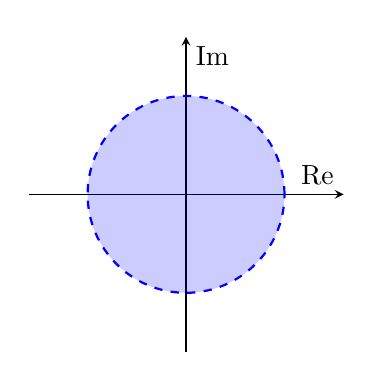
\begin{tikzpicture}
	\begin{axis}
	[
	axis y line=middle,
	axis x line=middle,
	xlabel = {Re},
	ylabel = {Im},
	xtick style={draw=none},
	ytick style={draw=none},
	y=1cm/1,
	x=1cm/1,
	xmin=-2,
	xmax=2,
	ymin=-2,
	ymax=2,
	yticklabels={,,},
	xticklabels={,,},
	%			xtick={1},
	ticklabel style={xshift=0.7ex}
	]
	\draw [name path=A,dashed, blue, thick, fill = blue, fill opacity = .2](axis cs:0,0) circle [radius=1.25];
	%		\draw [name path=B,dashed, blue, thick](axis cs:0,0) circle [radius=.5];
	%		\addplot[blue, fill opacity=0.2] fill between[of=A and B];
	%			\draw [thick](axis cs:0,0) circle [radius=1];
	%			\draw [black, thick, fill = white](axis cs:2,0) circle [radius=.1];
	%			\draw (axis cs:-2,0) node {\Cross};
	\end{axis}
	\end{tikzpicture}
\end{figure}
	
	\column{.33\linewidth}
			\begin{figure}[h!]
		\centering
		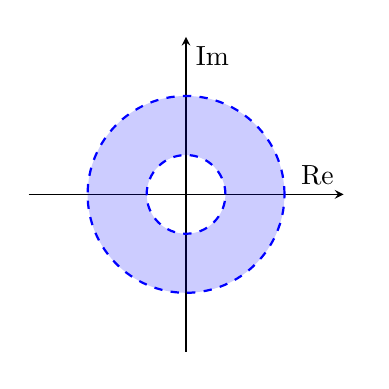
\begin{tikzpicture}
		\begin{axis}
		[
		axis y line=middle,
		axis x line=middle,
		xlabel = {Re},
		ylabel = {Im},
		xtick style={draw=none},
		ytick style={draw=none},
		y=1cm/1,
		x=1cm/1,
		xmin=-2,
		xmax=2,
		ymin=-2,
		ymax=2,
		yticklabels={,,},
		xticklabels={,,},
		%			xtick={1},
		ticklabel style={xshift=0.7ex}
		]
		\draw [name path=A,dashed, blue, thick](axis cs:0,0) circle [radius=1.25];
		\draw [name path=B,dashed, blue, thick](axis cs:0,0) circle [radius=.5];
		\addplot[blue, fill opacity=0.2] fill between[of=A and B];
		%			\draw [thick](axis cs:0,0) circle [radius=1];
		%			\draw [black, thick, fill = white](axis cs:2,0) circle [radius=.1];
		%			\draw (axis cs:-2,0) node {\Cross};
		\end{axis}
		\end{tikzpicture}
	\end{figure}

	\column{.33\linewidth}
\begin{figure}[h!]
	\centering
	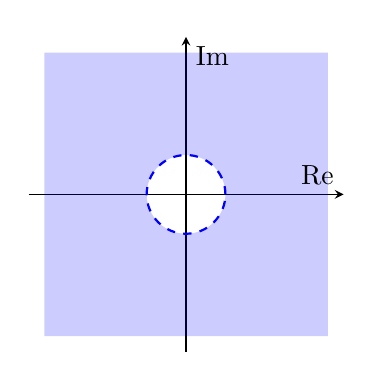
\begin{tikzpicture}
	\begin{axis}
	[
	axis y line=middle,
	axis x line=middle,
	xlabel = {Re},
	ylabel = {Im},
	xtick style={draw=none},
	ytick style={draw=none},
	y=1cm/1,
	x=1cm/1,
	xmin=-2,
	xmax=2,
	ymin=-2,
	ymax=2,
	yticklabels={,,},
	xticklabels={,,},
	%			xtick={1},
	ticklabel style={xshift=0.7ex}
	]
	\draw[name path = A, draw=none] (axis cs:-1.8,-1.8) rectangle (axis cs:1.8,1.8);
	\draw [name path=B,dashed, blue, thick](axis cs:0,0) circle [radius=.5];
	\addplot[blue, fill opacity=0.2] fill between[of=A and B];
	%			\draw [thick](axis cs:0,0) circle [radius=1];
	%			\draw [black, thick, fill = white](axis cs:2,0) circle [radius=.1];
	%			\draw (axis cs:-2,0) node {\Cross};
	\end{axis}
	\end{tikzpicture}
\end{figure}
		
	\end{columns}
\end{frame}

\begin{frame}{Properties of the ROC}
	\begin{block}{Property 2}
		The ROC does not contain any poles.
	\end{block}
\end{frame}

\begin{frame}{Properties of the ROC}
	\begin{block}{Property 3}
		If $ x[n] $ is of finite duration, then the ROC is the entire $ z $-plane, except possibly $ z=0 $ and/or $ z = \infty $.
	\end{block}
\[\begin{aligned}
	x_1[n] &= \delta[n] &\quad& X_1(z) = 1 &\quad&\mathrm{ROC}=\mathbb{C}\\
	x_2[n] &= \delta[n]+\delta[n-1] &\quad& X_2(z) = 1+z^{-1}&\quad&\mathrm{ROC}=\mathbb{C}-\{0\}\\
	x_3[n] &= \delta[n+1]+\delta[n] &\quad& X_3(z) = z+1&\quad&\mathrm{ROC}=\mathbb{C}-\{\infty\}\\
	x_4[n] &= \delta[n+1]+\delta[n]+\delta[n-1] &\quad& X_4(z) = z+1+z^{-1}&\quad&\mathrm{ROC}=\mathbb{C}-\{0,\infty\}
\end{aligned}\]
\end{frame}

\begin{frame}{Properties of the ROC}
	\begin{columns}
	\column{.66\linewidth}	
		\begin{block}{Property 4}
		If $ x[n] $ is a \textit{right-sided} sequence, and if the circle $ |z| = r_0 $ is in the ROC, then all finite values of $ z $ for which $ |z| > r_0 $ will also be in the ROC.
	\end{block}
	
	\begin{definition}
		The signal $ x[n] $ or $ x(t) $ is called \textbf{right-sided} if:
		\[\exists n_0 \: , \: \forall n < n_0 \: : \: x[n] = 0\]
		\[\exists t_0 \: , \:\forall t < t_0 \: : \: x(t) = 0\]
	\end{definition}
		
	\column{.33\linewidth}
		\begin{figure}[h!]
			\centering
			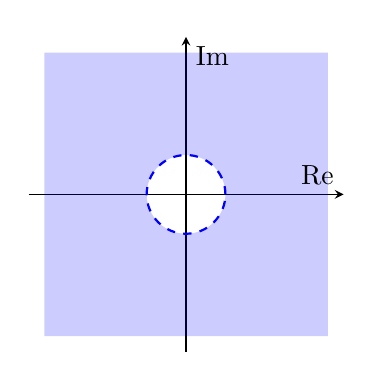
\begin{tikzpicture}
			\begin{axis}
			[
			axis y line=middle,
			axis x line=middle,
			xlabel = {Re},
			ylabel = {Im},
			xtick style={draw=none},
			ytick style={draw=none},
			y=1cm/1,
			x=1cm/1,
			xmin=-2,
			xmax=2,
			ymin=-2,
			ymax=2,
			yticklabels={,,},
			xticklabels={,,},
			%			xtick={1},
			ticklabel style={xshift=0.7ex}
			]
			\draw[name path = A, draw=none] (axis cs:-1.8,-1.8) rectangle (axis cs:1.8,1.8);
			\draw [name path=B,dashed, blue, thick](axis cs:0,0) circle [radius=.5];
			\addplot[blue, fill opacity=0.2] fill between[of=A and B];
			%			\draw [thick](axis cs:0,0) circle [radius=1];
			%			\draw [black, thick, fill = white](axis cs:2,0) circle [radius=.1];
			%			\draw (axis cs:-2,0) node {\Cross};
			\end{axis}
			\end{tikzpicture}
		\end{figure}
		
	\end{columns}

\end{frame}


\begin{frame}{Properties of the ROC}
	\begin{columns}
		\column{.66\linewidth}	
	\begin{block}{Property 5}
	If $ x[n] $ is a \textit{left-sided} sequence, and if the circle $ |z| = r_0 $ is in the ROC, then all values of $ z $ for which $ 0 < |z| < r_0 $ will also be in the ROC.
	\end{block}
	
	\begin{definition}
		The signal $ x[n] $ or $ x(t) $ is called \textbf{left-sided} if:
		\[\exists n_0 \: , \: \forall n > n_0 \: : \: x[n] = 0\]
		\[\exists t_0 \: , \:\forall t > t_0 \: : \: x(t) = 0\]
	\end{definition}

		
		\column{.33\linewidth}
		\begin{figure}
			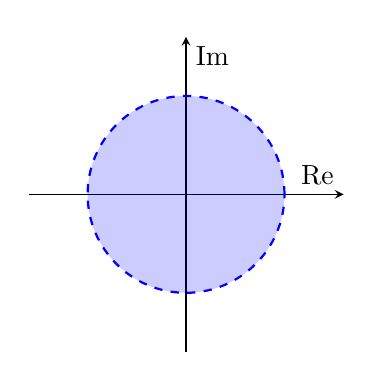
\begin{tikzpicture}
		\begin{axis}
		[
		axis y line=middle,
		axis x line=middle,
		xlabel = {Re},
		ylabel = {Im},
		xtick style={draw=none},
		ytick style={draw=none},
		y=1cm/1,
		x=1cm/1,
		xmin=-2,
		xmax=2,
		ymin=-2,
		ymax=2,
		yticklabels={,,},
		xticklabels={,,},
		%			xtick={1},
		ticklabel style={xshift=0.7ex}
		]
		\draw [name path=A,dashed, blue, thick, fill = blue, fill opacity = .2](axis cs:0,0) circle [radius=1.25];
		%		\draw [name path=B,dashed, blue, thick](axis cs:0,0) circle [radius=.5];
		%		\addplot[blue, fill opacity=0.2] fill between[of=A and B];
		%			\draw [thick](axis cs:0,0) circle [radius=1];
		%			\draw [black, thick, fill = white](axis cs:2,0) circle [radius=.1];
		%			\draw (axis cs:-2,0) node {\Cross};
		\end{axis}
		\end{tikzpicture}
		\end{figure}
	\end{columns}
	
\end{frame}

\begin{frame}{Properties of the ROC}
	\begin{columns}
		\column{.66\linewidth}	
		\begin{block}{Property 6}
			If $ x[n] $ is two sided, and if the circle $ |z| = r_0 $ is in the ROC, then the ROC will consist of a ring in the $ z $-plane that includes the circle $ |z| = r_0 $.
		\end{block}
		
		
		\begin{definition}
			The signal $ x[n] $ or $ x(t) $ is called \textbf{two sided} if it is neither left-sided nor right-sided.
		\end{definition}
		
		
		\column{.33\linewidth}
		\begin{figure}[h!]
			\centering
			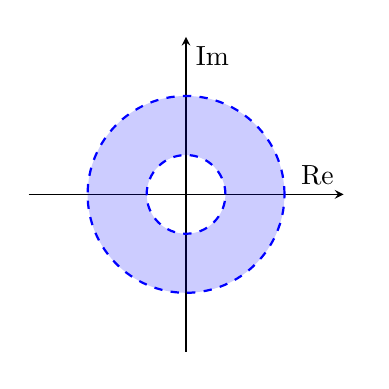
\begin{tikzpicture}
			\begin{axis}
			[
			axis y line=middle,
			axis x line=middle,
			xlabel = {Re},
			ylabel = {Im},
			xtick style={draw=none},
			ytick style={draw=none},
			y=1cm/1,
			x=1cm/1,
			xmin=-2,
			xmax=2,
			ymin=-2,
			ymax=2,
			yticklabels={,,},
			xticklabels={,,},
			%			xtick={1},
			ticklabel style={xshift=0.7ex}
			]
			\draw [name path=A,dashed, blue, thick](axis cs:0,0) circle [radius=1.25];
			\draw [name path=B,dashed, blue, thick](axis cs:0,0) circle [radius=.5];
			\addplot[blue, fill opacity=0.2] fill between[of=A and B];
			%			\draw [thick](axis cs:0,0) circle [radius=1];
			%			\draw [black, thick, fill = white](axis cs:2,0) circle [radius=.1];
			%			\draw (axis cs:-2,0) node {\Cross};
			\end{axis}
			\end{tikzpicture}
		\end{figure}
		
	\end{columns}
	
\end{frame}

\begin{frame}{Properties of the ROC}
	\begin{block}{Property 7}
		If the $ z $-transform $ X(z) $ of $ x[n] $ is rational, then its ROC is bounded by poles or extends to infinity.
	\end{block}
\end{frame}

\begin{frame}{Properties of the ROC}
	\begin{block}{Property 8}
		If the $ z $-transform $ X(z) $ of $ x[n] $ is rational, and if $ x[n] $ is right sided, then the ROC is the region in the $ z $-plane outside the outermost pole -- i.e., outside the circle of radius equal to the largest magnitude of the poles of $ X(z) $. Furthermore, if $ x[n] $ is
		causal (i.e., if it is right sided and equal to $ 0 $ for $ n < 0 $), then the ROC also includes $ z = \infty $.
	\end{block}
\end{frame}

\begin{frame}{Properties of the ROC}
	\begin{block}{Property 9}
		If the $ z $-transform $ X(z) $ of $ x[n] $ is rational, and if $ x[n] $ is left sided, then	the ROC is the region in the $ z $-plane inside the innermost nonzero pole -- i.e., inside the	circle of radius equal to the smallest magnitude of the poles of $ X(z) $ other than any at
		$ z = 0 $ and extending inward to and possibly including $ z = 0 $. In particular, if $ x[n] $ is \textit{anticausal} (i.e., if it is left sided and equal to $ 0 $ for $ n > 0 $), then the ROC also includes
		$ z = 0 $.
	\end{block}
\end{frame}

\begin{frame}{Example \#3}

	\[X(z)=\frac{z^2-\frac{3}{2}z}{z^2-\frac{5}{6}z+\frac{1}{6}}\Rightarrow x[n]=?\]
	\begin{columns}
		\column{.4\linewidth}
	\begin{align*}
		\only<2->{ X(z) &= \frac{z(z-\frac{3}{2})}{(z-\frac{1}{3})(z-\frac{1}{2})}\\}
		\only<3->{ &= \frac{7}{1-\frac{1}{3}z^{-1}}-\frac{6}{1-\frac{1}{2}z^{-1}}\\}
	\end{align*}
	\column{.05\linewidth}
	\only<5->{\[\Rightarrow\]}
	\column{.55\linewidth}
	\only<4>{
		\textbf{Do you remember the results from examples \#1 and \#2?}
	}
	\only<5->{
		\[x[n] = \begin{cases}
		7\left(\frac{1}{3}\right)^nu[n]-6\left(\frac{1}{2}\right)^nu[n] \\
		7\left(\frac{1}{3}\right)^nu[n]+6\left(\frac{1}{2}\right)^nu[-n-1] \\
		-7\left(\frac{1}{3}\right)^nu[-n-1]+6\left(\frac{1}{2}\right)^nu[-n-1]\\
		\textcolor{red}{-7\left(\frac{1}{3}\right)^nu[-n-1]-6\left(\frac{1}{2}\right)^nu[n]}
		\end{cases}\]
	}
	\end{columns}
\end{frame}

\begin{frame}{Example \#3}
\only<1>{
	\[X(z)=\frac{z(z-\frac{3}{2})}{(z-\frac{1}{3})(z-\frac{1}{2})}\Rightarrow x[n]=7\left(\frac{1}{3}\right)^nu[n]-6\left(\frac{1}{2}\right)^nu[n]\]
		\begin{figure}[h!]
			\centering
			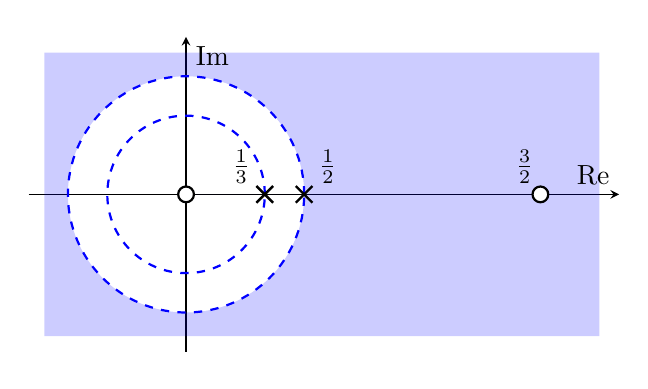
\begin{tikzpicture}
			\begin{axis}
			[
			axis y line=middle,
			axis x line=middle,
			xtick style={draw=none},
			ytick style={draw=none},
			xlabel = {Re},
			ylabel = {Im},
			y=1cm/1,
			x=1cm/1,
			xmin=-2,
			xmax=5.5,
			ymin=-2,
			yticklabels={,,},
			xticklabels={,,},
%			xtick={},
			ticklabel style={xshift=0.7ex},
			ymax=2
			]
			\draw[name path = C, draw=none] (axis cs:-1.8,-1.8) rectangle (axis cs:5.25,1.8);
			\draw [name path=A,dashed, blue, thick](axis cs:0,0) circle [radius=1.5];
			\draw [name path=B,dashed, blue, thick](axis cs:0,0) circle [radius=1];
			\addplot[blue, fill opacity=0.2] fill between[of=A and C];
%			\draw [thick](axis cs:0,0) circle [radius=1];
			\draw [black, thick, fill = white](axis cs:0,0) circle [radius=.1];
			\draw [black, thick, fill = white](axis cs:4.5,0) circle [radius=.1];
			\draw (axis cs:1.5,0) node {\Cross};
			\draw (axis cs:1,0) node {\Cross};
			\draw (axis cs:4.3,.35) node {$ \frac{3}{2} $};
			\draw (axis cs:1.8,.35) node {$ \frac{1}{2} $};
			\draw (axis cs:.7,.35) node {$ \frac{1}{3} $};
			\end{axis}
			\end{tikzpicture}
		\end{figure}
}
\only<2>{
	\[X(z)=\frac{z(z-\frac{3}{2})}{(z-\frac{1}{3})(z-\frac{1}{2})}\Rightarrow x[n]=7\left(\frac{1}{3}\right)^nu[n]+6\left(\frac{1}{2}\right)^nu[-n-1]
	\]
	\begin{figure}[h!]
		\centering
		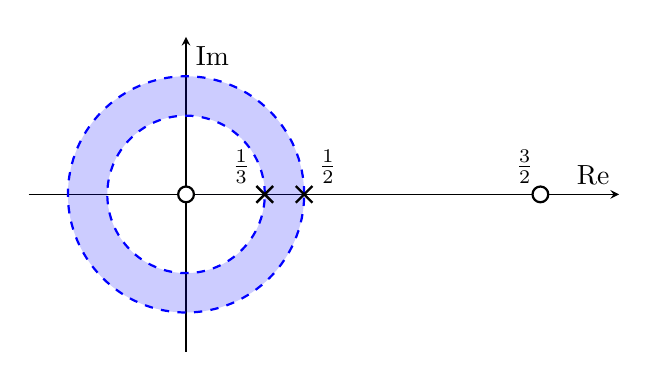
\begin{tikzpicture}
		\begin{axis}
		[
		axis y line=middle,
		axis x line=middle,
		xtick style={draw=none},
		ytick style={draw=none},
		xlabel = {Re},
		ylabel = {Im},
		y=1cm/1,
		x=1cm/1,
		xmin=-2,
		xmax=5.5,
		ymin=-2,
		yticklabels={,,},
		xticklabels={,,},
		%			xtick={},
		ticklabel style={xshift=0.7ex},
		ymax=2
		]
		\draw[name path = C, draw=none] (axis cs:-1.8,-1.8) rectangle (axis cs:5.25,1.8);
		\draw [name path=A,dashed, blue, thick](axis cs:0,0) circle [radius=1.5];
		\draw [name path=B,dashed, blue, thick](axis cs:0,0) circle [radius=1];
		\addplot[blue, fill opacity=0.2] fill between[of=A and B];
		%			\draw [thick](axis cs:0,0) circle [radius=1];
		\draw [black, thick, fill = white](axis cs:0,0) circle [radius=.1];
		\draw [black, thick, fill = white](axis cs:4.5,0) circle [radius=.1];
		\draw (axis cs:1.5,0) node {\Cross};
		\draw (axis cs:1,0) node {\Cross};
		\draw (axis cs:4.3,.35) node {$ \frac{3}{2} $};
		\draw (axis cs:1.8,.35) node {$ \frac{1}{2} $};
		\draw (axis cs:.7,.35) node {$ \frac{1}{3} $};
		\end{axis}
		\end{tikzpicture}
	\end{figure}
}
\only<3>{
	\[X(z)=\frac{z(z-\frac{3}{2})}{(z-\frac{1}{3})(z-\frac{1}{2})}\Rightarrow x[n]=-7\left(\frac{1}{3}\right)^nu[-n-1]+6\left(\frac{1}{2}\right)^nu[-n-1]\]
	\begin{figure}[h!]
		\centering
		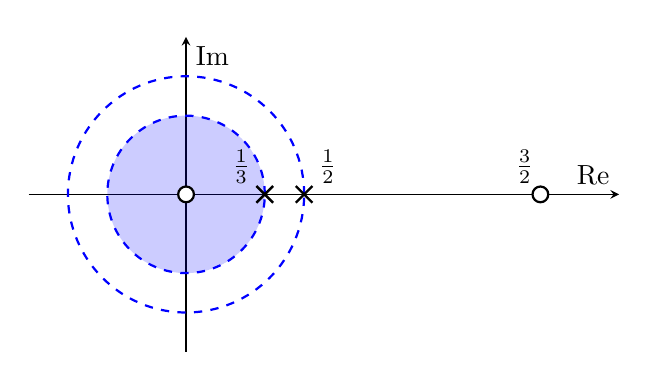
\begin{tikzpicture}
		\begin{axis}
		[
		axis y line=middle,
		axis x line=middle,
		xtick style={draw=none},
		ytick style={draw=none},
		xlabel = {Re},
		ylabel = {Im},
		y=1cm/1,
		x=1cm/1,
		xmin=-2,
		xmax=5.5,
		ymin=-2,
		yticklabels={,,},
		xticklabels={,,},
		%			xtick={},
		ticklabel style={xshift=0.7ex},
		ymax=2
		]
		\draw [name path=A,dashed, blue, thick](axis cs:0,0) circle [radius=1.5];
		\draw [name path=B,dashed, blue, thick, fill = blue, fill opacity = .2](axis cs:0,0) circle [radius=1];
		%			\draw [thick](axis cs:0,0) circle [radius=1];
		\draw [black, thick, fill = white](axis cs:0,0) circle [radius=.1];
		\draw [black, thick, fill = white](axis cs:4.5,0) circle [radius=.1];
		\draw (axis cs:1.5,0) node {\Cross};
		\draw (axis cs:1,0) node {\Cross};
		\draw (axis cs:4.3,.35) node {$ \frac{3}{2} $};
		\draw (axis cs:1.8,.35) node {$ \frac{1}{2} $};
		\draw (axis cs:.7,.35) node {$ \frac{1}{3} $};
		\end{axis}
		\end{tikzpicture}
	\end{figure}
}
\only<4>{
	\[X(z)=\frac{z(z-\frac{3}{2})}{(z-\frac{1}{3})(z-\frac{1}{2})}\Rightarrow x[n]=-7\left(\frac{1}{3}\right)^nu[-n-1]-6\left(\frac{1}{2}\right)^nu[n]\]
	\begin{figure}[h!]
		\centering
		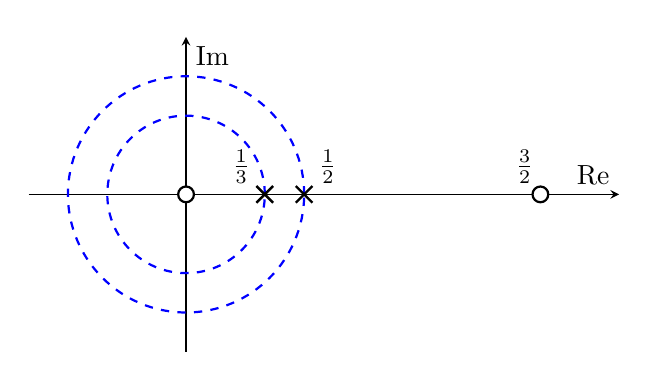
\begin{tikzpicture}
		\begin{axis}
		[
		axis y line=middle,
		axis x line=middle,
		xtick style={draw=none},
		ytick style={draw=none},
		xlabel = {Re},
		ylabel = {Im},
		y=1cm/1,
		x=1cm/1,
		xmin=-2,
		xmax=5.5,
		ymin=-2,
		yticklabels={,,},
		xticklabels={,,},
		%			xtick={},
		ticklabel style={xshift=0.7ex},
		ymax=2
		]
		\draw [name path=A,dashed, blue, thick](axis cs:0,0) circle [radius=1.5];
		\draw [name path=B,dashed, blue, thick](axis cs:0,0) circle [radius=1];
		%			\draw [thick](axis cs:0,0) circle [radius=1];
		\draw [black, thick, fill = white](axis cs:0,0) circle [radius=.1];
		\draw [black, thick, fill = white](axis cs:4.5,0) circle [radius=.1];
		\draw (axis cs:1.5,0) node {\Cross};
		\draw (axis cs:1,0) node {\Cross};
		\draw (axis cs:4.3,.35) node {$ \frac{3}{2} $};
		\draw (axis cs:1.8,.35) node {$ \frac{1}{2} $};
		\draw (axis cs:.7,.35) node {$ \frac{1}{3} $};
		\end{axis}
		\end{tikzpicture}
	\end{figure}
}
\end{frame}



\section{Properties of the $ z $-Transform}
\begin{frame}{Linearity}
	If\\
	 \[x_1[n] \xleftrightarrow[]{\quad\mathcal{Z}\quad} X_1(z) \text{, with } \mathrm{ROC} =R_1\]
	and\\
	\[ x_2[n] \xleftrightarrow[]{\quad\mathcal{Z}\quad} X_2(z) \text{, with   } \mathrm{ROC} =R_2 \]
	then
	\begin{block}{Property 1}
		\[ ax_1[n]+bx_2[n] \xleftrightarrow[]{\quad\mathcal{Z}\quad} aX_1(z)+bX_2(z)\]  
		\centering
		with ROC containing  $ R_1\cap R_2 $ 
	\end{block}
\end{frame}

\begin{frame}{Time Shifting}
	If\\
	\[x[n] \xleftrightarrow[]{\quad\mathcal{Z}\quad} X(z) \text{, with } \mathrm{ROC} =R\]
	then
	\begin{block}{Property 2}
		\[ x[n-n_0] \xleftrightarrow[]{\quad\mathcal{Z}\quad} z^{-n_0}X(z) \]
		\centering
		 with $\mathrm{ROC} = R $, except for the possible addition or deletion of the origin or infinity.
	\end{block}
\end{frame}

\begin{frame}{Scaling in the $ z $-domain}
	If\\
	\[x[n] \xleftrightarrow[]{\quad\mathcal{Z}\quad} X(z) \text{, with } \mathrm{ROC} =R\]
	then
	\begin{block}{Property 3}
		\[ z_0^nx[n] \xleftrightarrow[]{\quad\mathcal{Z}\quad} X\left(\frac{z}{z_0}\right) \]
		\centering
		with $\mathrm{ROC} = |z_0|R $
	\end{block}
\end{frame}

\begin{frame}{Time Reversal}
	If\\
	\[x[n] \xleftrightarrow[]{\quad\mathcal{Z}\quad} X(z) \text{, with } \mathrm{ROC} =R\]
	then
	\begin{block}{Property 4}
		\[ x[-n] \xleftrightarrow[]{\quad\mathcal{Z}\quad} X\left(\frac{1}{z}\right) \]
		\centering
		with $\mathrm{ROC} = \dfrac{1}{R} $
	\end{block}
\end{frame}

\begin{frame}{Time Expansion}
	If\\
	\[x[n] \xleftrightarrow[]{\quad\mathcal{Z}\quad} X(z) \text{, with } \mathrm{ROC} =R\]
	and
	\[x_{(k)}[n]=\begin{cases}
	x[n/k] & \text{if $ n $ is a multiple of $ k $}\\
	0 & \text{if $ n $ is not a multiple of $ k $}\\
	\end{cases}\]
	then
	\begin{block}{Property 5}
		\[ x_{(k)}[n] \xleftrightarrow[]{\quad\mathcal{Z}\quad} X(z^k) \]
		\centering
		with $\mathrm{ROC} = R^{1/k} $
	\end{block}
\end{frame}

\begin{frame}{Conjugation}
	If\\
	\[x[n] \xleftrightarrow[]{\quad\mathcal{Z}\quad} X(z) \text{, with } \mathrm{ROC} =R\]
	then
	\begin{block}{Property 6}
		\[ x^*[n] \xleftrightarrow[]{\quad\mathcal{Z}\quad} X^*(z^*) \]
		\centering
		with $\mathrm{ROC} = R $
	\end{block}
\end{frame}

\begin{frame}{The Convolution Property}
	If\\
	\[x_1[n] \xleftrightarrow[]{\quad\mathcal{Z}\quad} X_1(z) \text{, with } \mathrm{ROC} =R_1\]
	and\\
	\[ x_2[n] \xleftrightarrow[]{\quad\mathcal{Z}\quad} X_2(z) \text{, with   } \mathrm{ROC} =R_2 \]
	then
	\begin{block}{Property 7}
		\[ x_1[n]*x_2[n] \xleftrightarrow[]{\quad\mathcal{Z}\quad} X_1(z)X_2(z) \]
		\centering
		with ROC containing  $ R_1\cap R_2 $ 	
	\end{block}
\end{frame}

\begin{frame}{Differentiation in the $ z $-Domain}
	If\\
	\[x[n] \xleftrightarrow[]{\quad\mathcal{Z}\quad} X(z) \text{, with } \mathrm{ROC} =R\]
	then
	\begin{block}{Property 8}
		\[ nx[n] \xleftrightarrow[]{\quad\mathcal{Z}\quad} -z\dfrac{\mathrm{d}X(z)}{\mathrm{d}z} \]
		\centering
		with $\mathrm{ROC} = R $
	\end{block}
\end{frame}

\begin{frame}{Difference}
	If\\
	\[x[n] \xleftrightarrow[]{\quad\mathcal{Z}\quad} X(z) \text{, with } \mathrm{ROC} =R\]
	then
	\begin{block}{Property 9}
		\[ x[n]-x[n-1] \xleftrightarrow[]{\quad\mathcal{Z}\quad} (1-z^{-1})X(z) \]
		\centering
		with ROC containing $R\cap\{|z|>0\}$
	\end{block}
\end{frame}

\begin{frame}{Accumulation}
	If\\
	\[x[n] \xleftrightarrow[]{\quad\mathcal{Z}\quad} X(z) \text{, with } \mathrm{ROC} =R\]
	then
	\begin{block}{Property 10}
		\[ \sum_{k=-\infty}^{n}x[k] \xleftrightarrow[]{\quad\mathcal{Z}\quad} \dfrac{X(z)}{1-z^{-1}} \]
		\centering
		with ROC containing $R\cap\{|z|>1\}$
	\end{block}
\end{frame}

\begin{frame}{The Initial-Value Theorem}
	\begin{block}{Property 11}
			If 	$ \forall n<0\: : \: x[n]=0 $	then:
		\[	x[0] = \lim\limits_{z\to\infty}X(z)\]
	\end{block}
	Also we can find $ x[n] $ for larger values of $ n $ similarly:
	\[\begin{aligned}
	x[1] &= \lim\limits_{z\to\infty}z\left(X(z)-x[0]\right)\\
	x[2] &= \lim\limits_{z\to\infty}z^2\left(X(z)-x[0]-x[1]z^{-1}\right)\\
	x[3] &= \lim\limits_{z\to\infty}z^3\left(X(z)-x[0]-x[1]z^{-1}-x[2]z^{-2}\right)\\
	x[4] &= \lim\limits_{z\to\infty}z^4\left(X(z)-x[0]-x[1]z^{-1}-x[2]z^{-2}-x[3]z^{-3}\right)\\
	\dots & 
	\end{aligned}\]
\end{frame}

\begin{frame}{The Final-Value Theorem}
	\begin{block}{Property 12}
		If $ x[n] $ is right-handed and $ \lim\limits_{n\to\infty} x[n] $ exists, then:
		\[\lim\limits_{n\to\infty}x[n] = \lim\limits_{z\to1} (1-z^{-1})X(z)\]
	\end{block}
\end{frame}

\begin{frame}{Example \#4}
	\[X(z) = \frac{3z^{-3}}{\left(1-\frac{1}{4}z^{-1}\right)^2} \Rightarrow x[n] = ? \quad,\quad x[n]\text{ is left-sided}\]
	\begin{align*}
		\only<2->{
			\frac{1}{1-\frac{1}{4}z^{-1}} &\xleftrightarrow[]{\quad\mathcal{Z}\quad} -\left(\frac{1}{4}\right)^nu[-n-1]\\}
		\only<3->{
			-z\frac{\mathrm{d}}{\mathrm{d}z}\left(\frac{1}{1-\frac{1}{4}z^{-1}}\right) =  \frac{\frac{1}{4}z^{-1}}{\left(1-\frac{1}{4}z^{-1}\right)^2}
			&\xleftrightarrow[]{\quad\mathcal{Z}\quad} -n\left(\frac{1}{4}\right)^nu[-n-1]\\}
		\only<4->{
			12z^{-2}\left(-z\frac{\mathrm{d}}{\mathrm{d}z}\left(\frac{1}{1-\frac{1}{4}z^{-1}}\right)\right) =  \frac{3z^{-3}}{\left(1-\frac{1}{4}z^{-1}\right)^2}
			&\xleftrightarrow[]{\quad\mathcal{Z}\quad} -12(n-2)\left(\frac{1}{4}\right)^{(n-2)}u[-n+1]\\}
	\end{align*}
\end{frame}

\section{$ z $-Transform and LTI Systems}
\begin{frame}{System Transfer Function}
	The input-output relationship for an LTI system with impulse response $ h[n] $:
	\[y[n] = h[n]*x[n]\]
	Using the convolution property of the $ z $-transform:
	\[Y(z) = H(z)X(z)\]
	\[H(z) = \frac{Y(z)}{X(z)}\]
	\begin{block}{Definition}
		$ H(z) $ is called the \textbf{transfer function} (or \textbf{system function}) of the system.
	\end{block}
	Note that $ H(z) $ is the $ z $-transform of the impulse response of the system.
\end{frame}

\begin{frame}{Causality of LTI Systems}
	\begin{block}{Theorem}
		A discrete-time LTI system is causal if and only if the ROC of its system function is	the exterior of a circle, \textit{including infinity}.
	\end{block}

	\begin{block}{Theorem}
		A discrete-time LTI system with rational system function $ H(z) $ is causal if and only if:
		\begin{enumerate}[label=(\alph*)]
			\item the ROC is the exterior of a circle outside the outermost pole.
			\item with $ H(z) $	expressed as a ratio of polynomials in $ z $, the order of the numerator cannot be greater than the order of the denominator. 
		\end{enumerate}
	\end{block}
	\end{frame}

	\begin{frame}{Stability of LTI Systems}
		\begin{block}{Theorem}
			An LTI system is stable if and only if the ROC of its system function $ H(z) $ includes the unit circle, $ |z| = 1 $.
		\end{block}	
	\end{frame}

	\begin{frame}{Example \#5}
		\only<1>{
		Find the impulse response of the system described by the difference equation
		\[y[n]-\frac{5}{2}y[n-1]+y[n-2] = 2x[n] - \frac{5}{2}x[n-1]\]
		if the system is:
		\begin{enumerate}[label=(\alph*)]
			\item causal.
			\item stable.
			\item non-causal and unstable.
		\end{enumerate}}
		\only<2-4>{
		\[y[n]-\frac{5}{2}y[n-1]+y[n-2] = 2x[n] - \frac{5}{2}x[n-1]\]
		\[Y(z)-\frac{5}{2}z^{-1}Y(z)+z^{-2}Y(z) = 2X(z) - \frac{5}{2}z^{-1}X(z)\]
	}
\only<3-4>{
	\begin{align*}
		\only<3-4>{
			H(z) = \frac{Y(z)}{X(z)} &= \frac{2-\frac{5}{2}z^{-1}} {1-\frac{5}{2}z^{-1}+z^{-2}}\\
		}
		\only<4-4>{ &= \frac{1}{1-\frac{1}{2}z^{-1}} + \frac{1}{1-2z^{-1}}}
	\end{align*}
}
%\end{frame}
%\begin{frame}
	\only<5>{
		\begin{columns}
			\column{.5\textwidth}
			For a causal system:
			\[H(z) = \frac{1}{1-\frac{1}{2}z^{-1}} + \frac{1}{1-2z^{-1}}\]
			\[h[n] = \left(\frac{1}{2}\right)^nu[n] + 2^nu[n]\]
			
			\column{.5\textwidth}
				\begin{figure}[h!]
				\centering
				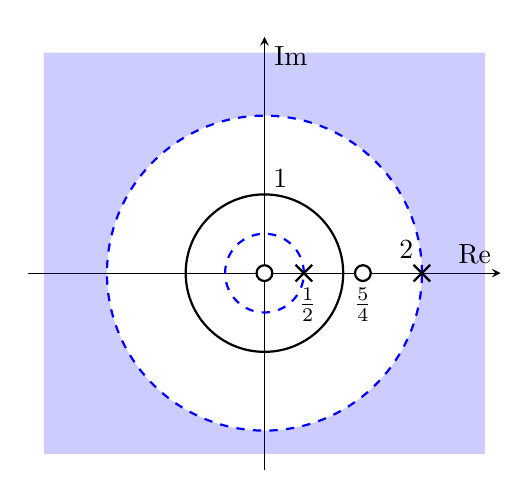
\begin{tikzpicture}
				\begin{axis}
				[
				axis y line=middle,
				axis x line=middle,
				xtick style={draw=none},
				ytick style={draw=none},
				xlabel = {Re},
				ylabel = {Im},
				y=1cm/1,
				x=1cm/1,
				xmin=-3,
				xmax=3,
				ymin=-2.5,
				yticklabels={,,},
				xticklabels={,,},
				%			xtick={},
				ticklabel style={xshift=0.7ex},
				ymax=3
				]
				\draw[name path = C, draw=none] (axis cs:-2.8,-2.3) rectangle (axis cs:2.8,2.8);
				\draw [name path=A,dashed, blue, thick](axis cs:0,0) circle [radius=2];
				\draw [name path=B,dashed, blue, thick](axis cs:0,0) circle [radius=.5];
				\draw [black, thick](axis cs:0,0) circle [radius=1];
				%			\draw [thick](axis cs:0,0) circle [radius=1];
				\draw [black, thick, fill = white](axis cs:0,0) circle [radius=.1];
				\draw [black, thick, fill = white](axis cs:1.25,0) circle [radius=.1];
				\addplot[blue, fill opacity=0.2] fill between[of=C and A];
				\draw (axis cs:2,0) node {\Cross};
				\draw (axis cs:.5,0) node {\Cross};
				\draw (axis cs:.55,-.4) node {$ \frac{1}{2} $};
				\draw (axis cs:1.25,-.4) node {$ \frac{5}{4} $};
				\draw (axis cs:1.8,.3) node {$ 2 $};
				\draw (axis cs:.2,1.2) node {$ 1 $};
				\end{axis}
				\end{tikzpicture}
			\end{figure}
		\end{columns}
	}

	\only<6>{
	\begin{columns}
		\column{.5\textwidth}
		For a stable system:
		\[H(z) = \frac{1}{1-\frac{1}{2}z^{-1}} + \frac{1}{1-2z^{-1}}\]
		\[h[n] = \left(\frac{1}{2}\right)^nu[n] - 2^nu[-n-1]\]
		
		\column{.5\textwidth}
		\begin{figure}[h!]
			\centering
			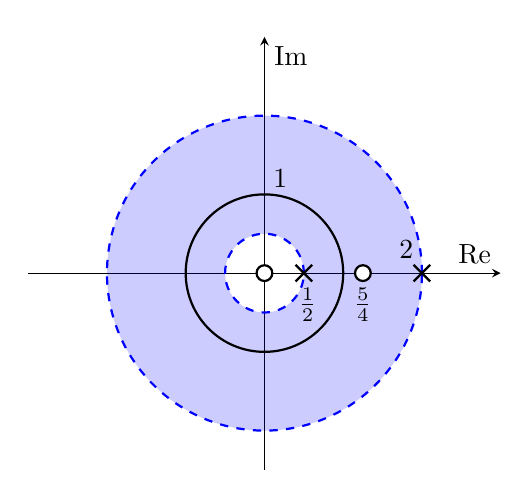
\begin{tikzpicture}
			\begin{axis}
			[
			axis y line=middle,
			axis x line=middle,
			xtick style={draw=none},
			ytick style={draw=none},
			xlabel = {Re},
			ylabel = {Im},
			y=1cm/1,
			x=1cm/1,
			xmin=-3,
			xmax=3,
			ymin=-2.5,
			yticklabels={,,},
			xticklabels={,,},
			%			xtick={},
			ticklabel style={xshift=0.7ex},
			ymax=3
			]
%			\draw[name path = C, draw=none] (axis cs:-2.8,-2.3) rectangle (axis cs:2.8,2.8);
			\draw [name path=A,dashed, blue, thick](axis cs:0,0) circle [radius=2];
			\draw [name path=B,dashed, blue, thick](axis cs:0,0) circle [radius=.5];
			\draw [black, thick](axis cs:0,0) circle [radius=1];
			%			\draw [thick](axis cs:0,0) circle [radius=1];
			\draw [black, thick, fill = white](axis cs:0,0) circle [radius=.1];
			\draw [black, thick, fill = white](axis cs:1.25,0) circle [radius=.1];
			\addplot[blue, fill opacity=0.2] fill between[of=B and A];
			\draw (axis cs:2,0) node {\Cross};
			\draw (axis cs:.5,0) node {\Cross};
			\draw (axis cs:.55,-.4) node {$ \frac{1}{2} $};
			\draw (axis cs:1.25,-.4) node {$ \frac{5}{4} $};
			\draw (axis cs:1.8,.3) node {$ 2 $};
			\draw (axis cs:.2,1.2) node {$ 1 $};
			\end{axis}
			\end{tikzpicture}
		\end{figure}
	\end{columns}
}

	\only<7>{
	\begin{columns}
		\column{.5\textwidth}
		For a non-causal and unstable system:
		\[H(z) = \frac{1}{1-\frac{1}{2}z^{-1}} + \frac{1}{1-2z^{-1}}\]
		\[h[n] = -\left(\frac{1}{2}\right)^nu[-n-1] - 2^nu[-n-1]\]
		
		\column{.5\textwidth}
		\begin{figure}[h!]
			\centering
			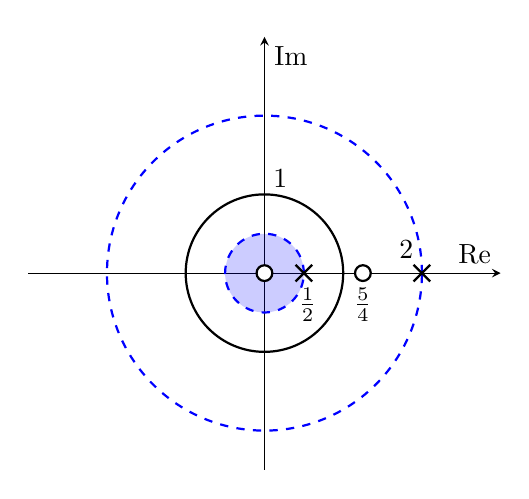
\begin{tikzpicture}
			\begin{axis}
			[
			axis y line=middle,
			axis x line=middle,
			xtick style={draw=none},
			ytick style={draw=none},
			xlabel = {Re},
			ylabel = {Im},
			y=1cm/1,
			x=1cm/1,
			xmin=-3,
			xmax=3,
			ymin=-2.5,
			yticklabels={,,},
			xticklabels={,,},
			%			xtick={},
			ticklabel style={xshift=0.7ex},
			ymax=3
			]
%			\draw[name path = C, draw=none] (axis cs:-2.8,-2.3) rectangle (axis cs:2.8,2.8);
			\draw [name path=A,dashed, blue, thick](axis cs:0,0) circle [radius=2];
			\draw [name path=B,dashed, blue, thick, fill = blue, fill opacity = .2](axis cs:0,0) circle [radius=.5];
			\draw [black, thick](axis cs:0,0) circle [radius=1];
			%			\draw [thick](axis cs:0,0) circle [radius=1];
			\draw [black, thick, fill = white](axis cs:0,0) circle [radius=.1];
			\draw [black, thick, fill = white](axis cs:1.25,0) circle [radius=.1];
%			\addplot[blue, fill opacity=0.2] fill between[of=C and A];
			\draw (axis cs:2,0) node {\Cross};
			\draw (axis cs:.5,0) node {\Cross};
			\draw (axis cs:.55,-.4) node {$ \frac{1}{2} $};
			\draw (axis cs:1.25,-.4) node {$ \frac{5}{4} $};
			\draw (axis cs:1.8,.3) node {$ 2 $};
			\draw (axis cs:.2,1.2) node {$ 1 $};

			\end{axis}
			\end{tikzpicture}
		\end{figure}
	\end{columns}
}
	\end{frame}


\end{document}